\documentclass{beamer}

\usepackage{graphicx}
\graphicspath{{../02_outputs/figures/}}
\def\accBase{79.98\%}
\def\f1Base{0.00\%}
\def\sensBase{0.00\%}
\def\espBase{100.00\%}

% Estilo de la presentación
\usetheme{Madrid}

% Información
\title{Predicción de pobreza}
\subtitle{Problem Set 2}
\author{Andrés Silva, Valentina Vera \&{} Julián Herrera}
\date{\today}

\begin{document}

% Diapositiva 1: Portada %%%%%%%%%%%%%%%%%%%%%%%%%%%%%%%%%%%%%%%%%%%%%%%%%%%%%%
\begin{frame}
    \titlepage
\end{frame}


% Diapositiva 2: Prueba de grafico %%%%%%%%%%%%%%%%%%%%%%%%%%%%%%%%%%%%%%%%%%%
\begin{frame}{Distribución de pobreza}
    \centering
    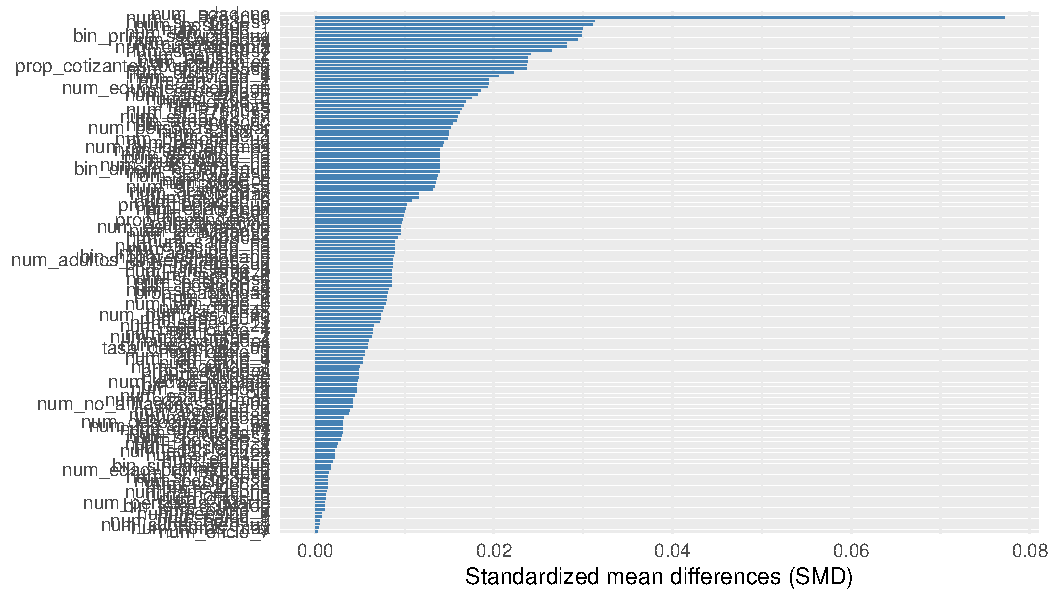
\includegraphics[width=0.85\textwidth]{SMD.pdf}
\end{frame}

% Diapositiva 3: Prueba de tabla %%%%%%%%%%%%%%%%%%%%%%%%%%%%%%%%%%%%%%%%%%%%


\begin{frame}{Baseline: Clasificador ingenuo}

\begin{block}{Estrategia}
Se clasifica a todos los hogares como
\textbf{No pobres}, independientemente
de sus características.
\end{block}


\begin{table}
\centering
\begin{tabular}{lc}
\hline
\textbf{Métrica} & \textbf{Resultado} \\
\hline
Accuracy       & \accBase \\
F1-score       & \f1Base \\
Sensibilidad   & \textbf{\sensBase} \\
Especificidad  & \espBase \\
\hline
\end{tabular}
\end{table}


\begin{alertblock}{Conclusión}
Un accuracy cercano al 80\% no garantiza
un buen desempeño: el clasificador
no identifica ningún hogar pobre.
\end{alertblock}

\end{frame}

\end{document}
